\documentclass[tikz,border=2mm]{standalone}
\usepackage{luatex85}
\usepackage{fontspec}
\usepackage{xcolor}
% Color palette — single source of truth
% Loaded by preamble.tex and build/images/standalone-header.tex

\definecolor{trackone}{HTML}{1A6B6A}    % Track 1 (Confession) — deep teal
\definecolor{tracktwo}{HTML}{C4913B}    % Track 2 (Testament) — warm amber
\definecolor{trackthree}{HTML}{6B3FA0}  % Track 3 (Awakening) — violet
\definecolor{coverbg}{HTML}{0D1117}     % Cover background — near-black
\definecolor{textprimary}{HTML}{E6EDF3} % Text on dark backgrounds
\definecolor{phfill}{HTML}{D0D0D0}      % Placeholder fill — gray
\definecolor{bodytext}{HTML}{1A1A1A}    % Body text — near-black
\definecolor{linkblue}{HTML}{2563EB}    % Link color — accessible blue
\definecolor{trackconv}{HTML}{8C7853}   % Convergence (all tracks) — warm bronze
\definecolor{trackbridge}{HTML}{808080}  % Bridge (meta/hybrid) — neutral gray



\begin{document}
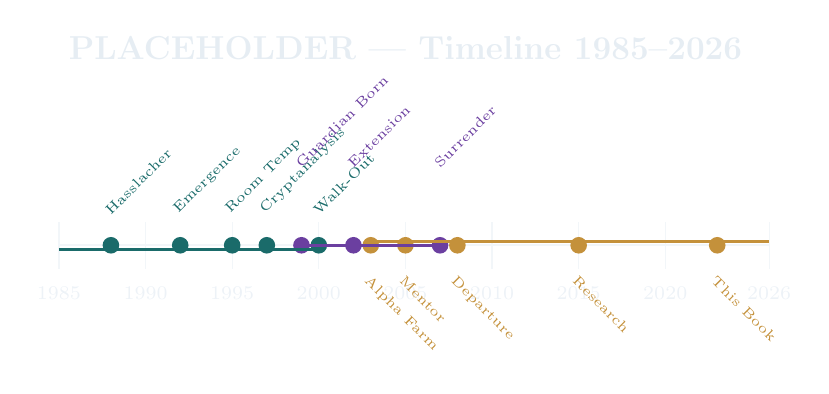
\begin{tikzpicture}[x=0.22cm]

% Title
\node[textprimary, font=\large\bfseries] at (20, 2.5) {PLACEHOLDER --- Timeline 1985--2026};

% Axis
\draw[textprimary!50, thick] (0,0) -- (41,0);

% Year markers and labels
\foreach \year/\pos in {1985/0, 1990/5, 1995/10, 2000/15, 2005/20, 2010/25, 2015/30, 2020/35, 2026/41} {
  \draw[textprimary!50] (\pos, -0.3) -- (\pos, 0.3);
  \node[textprimary!70, font=\scriptsize, below] at (\pos, -0.4) {\year};
}

% Track 1 events (above axis) — teal
\foreach \pos/\label in {3/Hasslacher, 7/Emergence, 10/Room Temp, 12/Cryptanalysis, 15/Walk-Out} {
  \fill[trackone] (\pos, 0) circle (3pt);
  \node[trackone, font=\tiny, above, rotate=45, anchor=south west] at (\pos, 0.2) {\label};
}

% Track 2 events (below axis) — amber
\foreach \pos/\label in {18/Alpha Farm, 20/Mentor, 23/Departure, 30/Research, 38/This Book} {
  \fill[tracktwo] (\pos, 0) circle (3pt);
  \node[tracktwo, font=\tiny, below, rotate=-45, anchor=north west] at (\pos, -0.2) {\label};
}

% Track 3 events (above axis, offset) — violet
\foreach \pos/\label in {14/Guardian Born, 17/Extension, 22/Surrender} {
  \fill[trackthree] (\pos, 0) circle (3pt);
  \node[trackthree, font=\tiny, above, rotate=45, anchor=south west] at (\pos, 0.8) {\label};
}

% Track-colored segments on axis
\draw[trackone, very thick] (0, -0.05) -- (15, -0.05);
\draw[tracktwo, very thick] (18, 0.05) -- (41, 0.05);
\draw[trackthree, very thick] (14, 0) -- (22, 0);

\end{tikzpicture}
\end{document}
